\subsection{Niveau 3 - AllerVers}

\begin{center}
\begin{figure}[!h]
%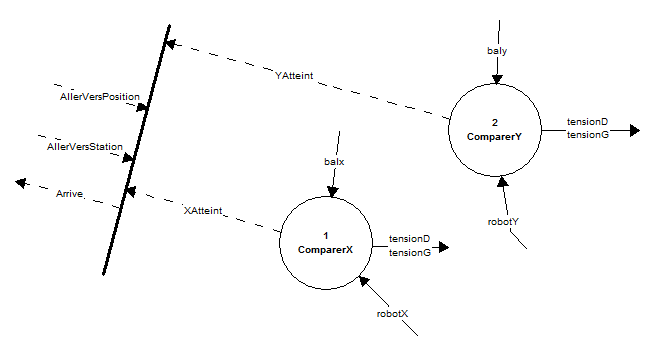
\includegraphics[scale=0.75]{\PIXPATH/allervers}
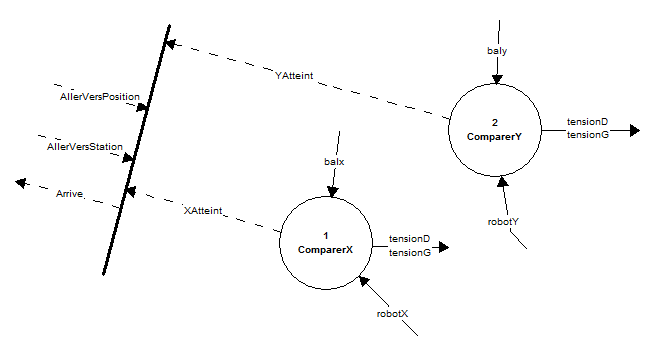
\includegraphics[height=8cm]{\PIXPATH/allervers}
\caption{Niveau 3 - AllerVers}
\end{figure}
\end{center}


\subsubsection{Diagramme états-transitions}

\begin{center}
\begin{figure}[!h]
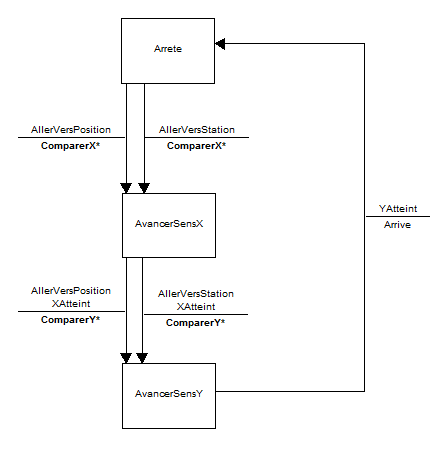
\includegraphics[height=10cm]{\PIXPATH/allervers_etat}
\caption{Diagramme états-transitions}
\end{figure}
\end{center}

\vfill
\pagebreak

\subsubsection{Processus primitifs - C-Spec}

\begin{description}
	
	\item \textbf{ComparerX}
		\begin{tabbing} 
		\textbf{IN} : robotX, balx \\
		\textbf{OUT} : tensionD, tensionG, XAtteint \\
		si \=($robotX \ge balx$) \\
			\>tensionD : 5 \\
			\>tensionG : 5 \\
		sinon si ($robotX \le balx$) \\ 
			\>tensionD : -5 \\
			\>tensionG : -5 \\
		sinon \\
			\>XAtteint emis \\
		fin si 
		\end{tabbing}

	\item \textbf{ComparerY}
		\begin{tabbing} 
		\textbf{IN} : robotY, baly \\
		\textbf{OUT} : tensionD, tensionG, YAtteint \\
		si \=($robotY \ge baly$) \\
			\>tensionD : 50 \\
			\>tensionG : 50 \\
		sinon si ($robotY \le baly$) \\
			\>tensionD : -50 \\
			\>tensionG : -50 \\
		sinon \\
			\>YAtteint emis \\
		fin si 
		\end{tabbing}


\end{description}

\vfill
\pagebreak

